\lab{Monte Carlo Integration}{Monte Carlo Integration}
\objective{Many important integrals cannot be evaluated symbolically because the integrand has no antiderivative.
Traditional numerical integration techniques like Newton-Cotes formulas and Gaussian quadrature usually work well for one-dimensional integrals, but rapidly become inefficient in higher dimensions.
Monte Carlo integration is an integration strategy that has relatively slow convergence, but that does extremely well in high-dimensional settings compared to other techniques.
In this lab we implement Monte Carlo integration and apply it to a classic problem in statistics.
}

% For example, the integral of the joint normal distribution
% \[
% \int_{\Omega} \frac{1}{\sqrt{(2 \pi)^k}} e^{- \frac{\bold{x}\trp\bold{x}}{2}}
% \]

\section*{Volume Estimation} % ================================================

Since the area of a circle of radius $r$ is $A = \pi r^2$, one way to numerically estimate $\pi$ is to compute the area of the unit circle.
Empirically, we can estimate the area by randomly choosing points in a domain that encompasses the unit circle.
The percentage of points that land within the unit circle approximates the percentage of the area of the domain that the unit circle occupies.
Multiplying this percentage by the total area of the sample domain gives an estimate for the area of the circle.

Since the unit circle has radius $r=1$, consider the square domain $\Omega=[-1,1]\times[-1,1]$.
The following code samples $2000$ uniformly distributed random points in $\Omega$, determines what percentage of those points are within the unit circle, then multiplies that percentage by $4$ (the area of $\Omega$) to get an estimate for $\pi$.

\begin{lstlisting}
>>> import numpy as np
>>> from scipy import linalg as la

# Get 2000 random points in the 2-D domain [-1,1]x[-1,1].
>>> points = np.random.uniform(-1, 1, (2,2000))

# Determine how many points are within the circle.
>>> lengths = la.norm(points, axis=0)
>>> num_within = np.count_nonzero(lengths < 1)

# Estimate the circle's area.
>>> 4 * (num_within / 2000)
3.198
\end{lstlisting}

The estimate $\pi \approx 3.198$ isn't perfect, but it only differs from the true value of $\pi$ by about $0.0564$.
On average, increasing the number of sample points decreases the estimate error.

\begin{figure}[H] % Estimating pi.
\captionsetup[subfigure]{justification=centering}
\centering
\begin{subfigure}{.32\textwidth}
    \centering
    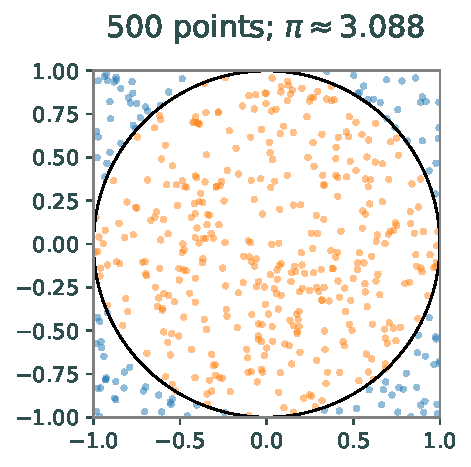
\includegraphics[width=\textwidth]{figures/mc_circle_0500.pdf}
\end{subfigure}
%
\begin{subfigure}{.32\textwidth}
    \centering
    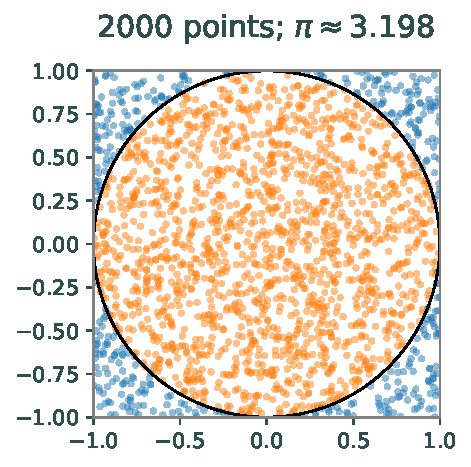
\includegraphics[width=\textwidth]{figures/mc_circle_2000.pdf}
\end{subfigure}
%
\begin{subfigure}{.32\textwidth}
    \centering
    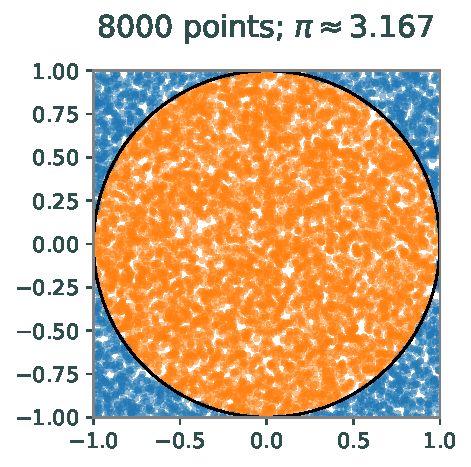
\includegraphics[width=\textwidth]{figures/mc_circle_8000.pdf}
\end{subfigure}
\caption{Estimating the area of the unit circle using random points.}
\end{figure}

\begin{problem}
The $n$-dimensional \emph{open unit ball} is the set $U_n = \{\x\in\mathbb{R}^n\mid \|\x\|_2 < 1\}$.
Write a function that accepts an integer $n$ and a keyword argument $N$ defaulting to $10^4$.
Estimate the volume of $U_n$ by drawing $N$ points over the $n$-dimensional domain $[-1,1]\times[-1,1]\times\cdots\times[-1,1]$.
\\(Hint: the volume of $[-1,1]\times[-1,1]\times\cdots\times[-1,1]$ is $2^n$.)

When $n=2$, this is the same experiment outlined above so your function should return an approximation of $\pi$.
The volume of the $U_3$ is $\frac{4}{3}\pi \approx 4.18879$, and the volume of $U_4$ is $\frac{\pi^2}{2} \approx 4.9348$.
Try increasing the number of sample points $N$ to see if your estimates improve.
\label{prob:unit-ball-volume}
\end{problem}

\section*{Integral Estimation} % ==============================================

The strategy for estimating $\pi$ can be formulated as an integral problem.
Define $f:\mathbb{R}^2\rightarrow\mathbb{R}$ by
\[
f(\x) =
\begin{cases}
1 &\mbox{ if $\|\x\|_2 < 1$ ($\x$ is within the unit circle)} \\
0 &\mbox{ otherwise,}
\end{cases}
\]
and let $\Omega = [-1,1] \times [-1,1]$ as before.
Then
\[
\int_{-1}^1\int_{-1}^1 f(x,y)\:dx\:dy = \int_\Omega f(\x)\:dV = \pi.
\]
To estimate the integral we chose $N$ random points $\{\x_i\}_{i=1}^N$ in $\Omega$.
Since $f$ indicates whether or not a point lies within the unit circle, the total number of random points that lie in the circle is the sum of the $f(\x_i)$.
Then the average of these values, multiplied by the volume $V(\Omega)$, is the desired estimate:
\begin{equation}
\int_\Omega f(\x)\:dV \approx V(\Omega) \frac{1}{N} \sum_{i=1}^N f(\x_i).
\label{eq:monte-carlo-integration}
\end{equation}
This remarkably simple equation can be used to estimate the integral of any integrable function $f:\mathbb{R}^n\rightarrow \mathbb{R}$ over any domain $\Omega \subset \mathbb{R}^n$ and is called the general formula for \emph{Monte Carlo integration}.

The intuition behind (\ref{eq:monte-carlo-integration}) is that $\frac{1}{N} \sum_{i=1}^N f(\x_i)$ approximates the average value of $f$ on $\Omega$, and multiplying the approximate average value by the volume of $\Omega$ yields the approximate integral of $f$ over $\Omega$.
This is a little easier to see in one dimension: for a single-variable function $f:\mathbb{R}\rightarrow\mathbb{R}$, the Average Value Theorem states that the average value of $f$ over an interval $[a,b]$ is given by
\[
f_{avg} = \frac{1}{b-a}\int_a^b f(x)\:dx.
\]
Then using the approximation $f_{avg} \approx \frac{1}{N} \sum_{i=1}^N f(x_i)$, the previous equation becomes
\begin{equation}
\int_a^b f(x)\:dx = (b - a) f_{avg} \approx V(\Omega)\frac{1}{N}\sum_{i=1}^N f(x_i),
\label{eq:monte-carlo-integration-1d}
\end{equation}
which is (\ref{eq:monte-carlo-integration}) in one dimension.
In this setting $\Omega = [a,b]$ and hence $V(\Omega) = b - a$.

\begin{problem}
Write a function that accepts a function $f:\mathbb{R}\rightarrow\mathbb{R}$, bounds of integration $a$ and $b$, and an integer $N$ defaulting to $10^4$.
Use \li{np.random.uniform()} to sample $N$ points over the interval $[a,b]$, then use (\ref{eq:monte-carlo-integration-1d}) to estimate the integral
\[
\int_a^b f(x)\:dx.
\]
Test your function on the following integrals, or on other integrals that you can check by hand.
\[
\begin{array}{c}
    \begin{array}{ccccc}
    \displaystyle\int_{-4}^2 x^2\:dx = 24
    & &
    \displaystyle\int_{-2\pi}^{2\pi} \sin(x)\:dx = 0
    & &
    \displaystyle\int_1^{10} \frac{1}{x}dx = \log(10) \approx 2.30259
    \end{array}
\\ \\
\displaystyle\int_1^5 \left|\sin(10x)\cos(10x) + \sqrt{x}\sin(3x) \right|\:dx \approx 4.502
\end{array}
\]
\label{prob:monte-carlo-integration-1d}
\end{problem}

\begin{warn}
Be careful not to use Monte Carlo integration to estimate integrals that do not converge.
For example, since $1/x$ approaches $\infty$ as $x$ approaches $0$ from the right, the integral \[\int_0^1 \frac{1}{x}\:dx\] does not converge.
Even so, attempts at Monte Carlo integration still return a finite value.
Use various numbers of sample points to see whether or not the integral estimate is converging.
\begin{lstlisting}
>>> for N in [5000, 7500, 10000]:
...     print(np.mean(1. / np.random.uniform(0, 1, N)), end='\t')
...
11.8451683722    25.5814419888    7.64364735049     # No convergence.
\end{lstlisting}
\end{warn}

\subsection*{Integration in Higher Dimensions} % ------------------------------

The implementation of (\ref{eq:monte-carlo-integration}) for a function $f:\mathbb{R}^n\rightarrow\mathbb{R}$ with $n > 1$ introduces a few tricky details, but the overall procedure is the same for the case when $n=1$.
We consider only the case where $\Omega \subset \mathbb{R}^n$ is an $n$-dimensional box $[a_1,b_1]\times[a_2,b_2]\times\cdots\times[a_n,b_n]$.
\begin{enumerate}
\item
If $n=1$ then $\Omega$ is a line, so $V(\Omega) = b_1 - a_1$.
If $n=2$ then $\Omega$ is a rectangle, and hence $V(\Omega) = (b_1 - a_1)(b_2-a_2)$, the product of the side lengths.
The volume of a higher-dimensional box $\Omega$ is also the product of the side lengths,
\begin{equation}
V(\Omega) = \prod_{i=1}^n (b_i - a_i)
\label{eq:mc-box-volume}
\end{equation}

\item It is easy to sample uniformly over an interval $[a,b]$ with \li{np.random.uniform()}, or even over the $n$-dimensional cube $[a,b]\times[a,b]\times\cdots\times[a,b]$ (such as in Problem \ref{prob:unit-ball-volume}).
However, if $a_i \ne a_j$ or $b_i \ne b_j$ for any $i\ne j$, the samples need to be constructed in a slightly different way.

The interval $[0,1]$ can be transformed to the interval $[a,b]$ by scaling it so that it is the same length as $[a,b]$, then shifting it to the appropriate location.
% \[((b - a) \cdot [0, 1]) + a = [0, b-a] + a = [a, b]\]
\[[0,1]\xrightarrow{\text{scale by } b-a} [0,b-a] \xrightarrow{\text{shift by } a} [a,b]\]
This suggests a strategy for sampling over $[a_1,b_1]\times[a_2,b_2]\times\cdots\times[a_n,b_n]$: sample uniformly from the $n$-dimensional box $[0, 1]\times[0, 1]\times\cdots\times[0, 1]$, multiply the $i$th component of each sample by $b_i - a_i$, then add $a_i$ to that component.
\begin{equation}
[0, 1]\times\cdots\times[0, 1]
\xrightarrow{\text{scale}}
[0, b_1-a_1]\times\cdots\times[0, b_n-a_n]
\xrightarrow{\text{shift}}
[a_1,b_1]\times\cdots\times[a_n,b_n]
\label{eq:mc-domain-transform}
\end{equation}
\end{enumerate}

\begin{problem}
Write a function that accepts a function $f:\mathbb{R}^n\rightarrow\mathbb{R}$, a list of lower bounds $[a_1, a_2, \ldots, a_n]$, a list of upper bounds $[b_1, b_2, \ldots, b_n]$, and an integer $N$ defaulting to $10^4$.
Use (\ref{eq:monte-carlo-integration}), (\ref{eq:mc-box-volume}), and (\ref{eq:mc-domain-transform}) with $N$ sample points to estimate the integral
\[
\int_\Omega f(\x)\:dV,
\]
where $\Omega = [a_1,b_1]\times[a_2,b_2]\times\cdots\times[a_n,b_n]$.
\\(Hint: use a list comprehension to calculate all of the $f(\x_i)$ quickly.)

Test your function on the following integrals.
\[
\begin{array}{c}
    \begin{array}{ccc}
    \displaystyle\int_0^1\int_0^1 x^2 + y^2\:dx\:dy = \frac{2}{3}
    & &
    \displaystyle\int_{-2}^1\int_1^3 3x - 4y + y^2\:dx\:dy = 54
    \end{array}
\\ \\
\displaystyle\int_{-4}^4\int_{-3}^3\int_{-2}^2\int_{-1}^1 x + y - w z^2\:dx\:dy\:dz\:dw = 0
\end{array}
\]
Note carefully how the order of integration defines the domain; in the last example, the $x$-$y$-$z$-$w$ domain is $[-1,1]\times[-2,2]\times[-3,3]\times[-4,4]$, so the lower and upper bounds passed to your function should be $[-1, -2, -3, -4]$ and $[1, 2, 3, 4]$, respectively.
% (this integral requires a very high $N$ for a good estimate)
\label{prob:montecarlo-integration-nd}
\end{problem}

\section*{Convergence} % ======================================================

Monte Carlo integration has some obvious pros and cons.
On the one hand, it is difficult to get highly precise estimates.
In fact, the error of the Monte Carlo method is proportional to $1/\sqrt{N}$, where $N$ is the number of points used in the estimation.
This means that dividing the error by $10$ requires using $100$ times more sample points.

On the other hand, the convergence rate is independent of the number of dimensions of the problem.
That is, the error converges at the same rate whether integrating a $2$-dimensional function or a $20$-dimensional function.
This gives Monte Carlo integration a huge advantage over other methods, and makes it especially useful for estimating integrals in high dimensions where other methods become computationally infeasible.

\begin{problem}
The probability density function of the joint distribution of $n$ independent normal random variables, each with mean $0$ and variance $1$, is the function $f:\mathbb{R}^n\rightarrow\mathbb{R}$ defined by
\[
f(\x) = \frac{1}{(2 \pi)^{n/2}} e^{- \frac{\x\trp\x}{2}}.
\]
% The integral of $f$ over a domain $\Omega\subset\mathbb{R}^n$ is the probability that a draw from the distribution will be in $\Omega$.
Though this is a critical distribution in statistics, $f$ does not have a symbolic antiderivative.

Integrate $f$ several times to study the convergence properties of Monte Carlo integration.

\begin{enumerate}
\item Let $n=4$ and $\Omega=[-\frac{3}{2}, \frac{3}{4}]\times[0,1]\times[0, \frac{1}{2}]\times[0,1] \subset \mathbb{R}^4$.
Define $f$ and $\Omega$ so that you can integrate $f$ over $\Omega$ using your function from Problem \ref{prob:montecarlo-integration-nd}.

\item Use \li{scipy.stats.mvn.mvnun()} to get the ``exact'' value of $F = \int_\Omega f(\x)\:dV$.
As an example, the following code computes the integral over $[-1,1]\times [-1,3]\times[-2,1] \subset \mathbb{R}^3$.
\begin{lstlisting}
>>> from scipy import stats

# Define the bounds of integration.
>>> mins = np.array([-1, -1, -2])
>>> maxs = np.array([ 1,  3,  1])

# The distribution has mean 0 and covariance I (the nxn identity).
>>> means, cov = np.zeros(3), np.eye(3)

# Compute the integral with SciPy.
>>> stats.mvn.mvnun(mins, maxs, means, cov)[0]
0.4694277116055261
\end{lstlisting}

\item Use \li{np.logspace()} to get $20$ \textbf{integer} values of $N$ that are roughly logarithmically spaced from $10^1$ to $10^5$.
For each value of $N$, use your function from Problem \ref{prob:montecarlo-integration-nd} to compute an estimate $\tilde{F}(N)$ of the integral with $N$ samples.
Compute the relative error $\frac{|F - \tilde{F}(N)|}{|F|}$ for each value of $N$.

\item Plot the relative error against the sample size $N$ on a log-log scale.
Also plot the line $1/\sqrt{N}$ for comparison.
Your results should be similar to Figure \ref{fig:monte-carlo-convergence}.
\end{enumerate}
\end{problem}

\begin{figure}[H] % Convergence of MC Integration.
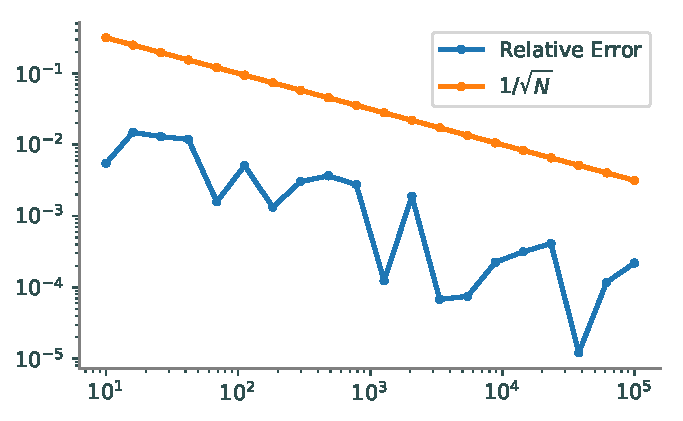
\includegraphics[width=.7\textwidth]{figures/mc_convergence.pdf}
\caption{Monte Carlo integration converges at the same rate as $1/\sqrt{N}$ where $N$ is the number of samples used in the estimate.
However, the convergence is independent of dimension, which is why this strategy is so commonly used for high-dimensional integration.
}
\label{fig:monte-carlo-convergence}
\end{figure}

\begin{comment} % Turned out to not be very interesting.
\begin{problem}
Repeat the experiment of Problem \ref{prob:mc-point-convergence}, but fix $N=10^4$ and define $\Omega_n$ to be the $n$-dimensional cube $[-1,1]\times[-1,1]\times\cdots\times[-1,1]$.
For $n=5,10,20,\ldots,100$, redefine $f$ and $\Omega_n$ to fit the dimension, use SciPy to compute the correct value of the integral $F_n$, use your function from Problem \ref{} to estimate the integral, and compute the relative error.

Plot the dimension against the relative error.
\end{problem}
\end{comment}

\begin{comment}
\begin{problem}
Create a new function (based upon the function from Problem \ref{prob:montecarlo-integration-nd}) that uses a ``flawed'' random number generator that doesn't produce numbers between $-.95$ and $-1$.
Test your method on the function from Problem \ref{prob:mc_test}.
How bad is the error?
\label{prob:mc_flawed}
\end{problem}
\end{comment}

\begin{comment} % TODO

\newpage

\section*{Additional Material} % ==============================================

\subsection*{Volumes in High Dimensions} % ------------------------------------

It is difficult to gain intuition on how large or small an integral should be in a high-dimensional space.
Examining the size of the unit balls gives a little insight.
The volumes $V_n$ of the open unit balls $U_n$ satisfy the following recurrence relation.
\[
V_0 = 1, \qquad V_1 = 2, \qquad V_n = \frac{2\pi}{n}V_{n-2}\ \ \text{for}\ \ n > 1.
\]
The following figure plots the dimension $n$ against the exact volume $V_n$, using the recurrence relation.
This provides another way to check Problem \ref{prob:unit-ball-volume}.

\begin{figure}[H]
    \includegraphics[width=.7\textwidth]{figures/unit_volumes.pdf}
\end{figure}

% \begin{table}[H]
% \begin{tabular}{c|r}
% Dimension $n$ & Volume $V_n$ \\ \hline
% 0 & 1 \\
% 1 & 2 \\
% 2 & $\pi \approx 3.142$ \\
% 3 & $\frac{4}{3}\pi \approx 4.189$ \\
% 4 & $\frac{1}{2}\pi^2 \approx 4.935$ \\
% 5 & $\frac{8}{15}\pi^2 \approx 5.264$ \\
% 6 & $\frac{1}{6}\pi^3 \approx 5.168$ \\
% 7 & $\frac{16}{105}\pi^3 \approx 4.725$ \\
% 8 & $\frac{1}{24}\pi^4 \approx 4.059$ \\
% 9 & $\frac{32}{945}\pi^4 \approx 3.299$ \\
% 10 & $\frac{1}{120}\pi^5 \approx 2.550$ \\
% \end{tabular}
% \end{table}

Note that the volume of the unit ball increases until $n=5$, at which point the volume decreases.
This is interesting because although initially the notion of ``more dimensions'' seems to go with ``more space,'' the restriction $\|\x\|_2 < 1$ becomes more and more limiting.

\subsection*{Other Monte Carlo Methods} % -------------------------------------

The idea of using random sampling for computations is not unique to numerical integration.
For example, \emph{Markov Chain Monte Carlo} (MCMC) methods combine strategic random sampling with the theory of Markov Chains to create a way to sample from difficult distributions.
% TODO: overview of other Monte Carlo methods.
\end{comment}
